% Romer 11.22 --- solution fragment for hardest-solutions.tex (statement not reproduced).
% Law of motion, steady states, stability signs and simulations re-checked by check-11-22-6-16.py.
\problema{Romer 11.22}{Cagan with adaptive expectations}{p.~583}{Romer \S11.9}

\passo{Environment}{Notation of \S11.9: $m\equiv M/P$ (real balances), $g_M\equiv\dot M/M$,
$\pi\equiv\dot P/P$; $S^{\mathrm{MAX}}$ is the largest seignorage that can be collected in a steady
state. In our words, the two assumptions are: real balances always equal Cagan's demand evaluated at
\emph{expected} inflation, $m=Ce^{-b\pi^e}$ ($C,b>0$); expectations move toward actual inflation at
speed $\beta$, $\dot\pi^e=\beta(\pi-\pi^e)$, with $0<\beta<1/b$. As in the text, real purchases $G$
are financed entirely by money creation, so $S(t)=G$ at every date.}

\parte{a}
\passo{Real balances inherit the motion of expectations}{Taking logs, $\ln m(t)=\ln C-b\pi^e(t)$;
differentiating with respect to time,
\[ \frac{\dot m(t)}{m(t)}=-b\,\dot\pi^e(t). \tag{1} \]}

\passo{The financing constraint}{Seignorage is $S=\dot M/P=(\dot M/M)(M/P)=g_M m$, so $S=G$ gives
$g_M=G/m$. Since $m=M/P$, $\dot m/m=g_M-\pi$; hence, using (1),
\[ \pi(t)=g_M(t)-\frac{\dot m(t)}{m(t)}=\frac{G}{m(t)}+b\,\dot\pi^e(t). \tag{2} \]
At a given instant $\pi^e(t)$ is predetermined, and so is $m(t)=Ce^{-b\pi^e(t)}$; the two unknowns
are $\pi(t)$ and $\dot\pi^e(t)$, linked by (2) and by the adaptive rule.}

\passo{Solve the two equations}{Substituting (2) into $\dot\pi^e=\beta(\pi-\pi^e)$,
\[ \dot\pi^e=\beta\Big[\frac{G}{m}+b\,\dot\pi^e-\pi^e\Big]
\quad\Longrightarrow\quad (1-b\beta)\,\dot\pi^e=\beta\Big[\frac{G}{m}-\pi^e\Big]. \]
Because $b\beta<1$ we can divide by $1-b\beta>0$; substituting $m=Ce^{-b\pi^e}$ then gives
\[ \begin{aligned}
\dot\pi^e(t)&=\frac{\beta}{1-b\beta}\;\frac{G-\pi^e(t)\,m(t)}{m(t)}\\
&=\frac{\beta}{1-b\beta}\Big[\frac{G}{C}\,e^{b\pi^e(t)}-\pi^e(t)\Big]\equiv\Phi\big(\pi^e(t)\big).
\end{aligned} \tag{3} \]}

\passo{Actual inflation}{From the adaptive rule, $\pi=\pi^e+\dot\pi^e/\beta$; with (3),
\[ \pi(t)=\pi^e(t)+\frac{G/m(t)-\pi^e(t)}{1-b\beta}=\frac{G/m(t)-b\beta\,\pi^e(t)}{1-b\beta}. \tag{4} \]}

\passo{The same law of motion as (11.75)}{Write $\pi^e=(\ln C-\ln m)/b$ and combine (1) with (3):
\[ \frac{\dot m}{m}=-b\,\dot\pi^e=\frac{b\beta}{1-b\beta}\;\frac{1}{m}\Big[\frac{\ln C-\ln m}{b}\,m-G\Big], \]
which is exactly (11.75). The two models are one model: in \S11.9 define $x\equiv(\ln C-\ln m)/b$,
the inflation rate that would make current holdings desired; then (11.71) reads $\dot x=\beta(\pi-x)$,
an adaptive rule for $x$. Figures 11.9--11.10 are thus the phase diagrams of this problem in
$(\ln m,\dot m/m)$ space; since $(\ln m,\dot m/m)=(\ln C-b\pi^e,\,-b\dot\pi^e)$, the diagrams in
$(\pi^e,\dot\pi^e)$ below are those figures rotated by $180^\circ$ and rescaled.}

\armadilha{The book asks for $\dot\pi^e$ ``as a function of $\pi(t)$''. Read literally, the adaptive
rule already is one; the analogue of (11.75) gives the motion of the state variable in terms of the
state alone, which is (3) (the solution manual reads it the same way). $\pi$ cannot serve as the
argument: by (4), $d\pi/d\pi^e=b\,(g_M-\beta)/(1-b\beta)$ changes sign where $g_M=\beta$, so two values
of $\pi^e$ map into the same $\pi$. Dropping the term $b\dot\pi^e$ in (2), i.e.\ setting $g_M=\pi$ off
the steady state, loses the factor $1/(1-b\beta)$ and, with it, the role of $\beta<1/b$.}

\parte{b}
\passo{The sign of $\dot\pi^e$ is the sign of a seignorage gap}{In a steady state $\dot\pi^e=0$ gives
$\pi=\pi^e$ and $\dot m=0$ gives $g_M=\pi$, so seignorage is $\pi m=C\pi e^{-b\pi}\equiv S(\pi)$, the
Laffer curve (11.68). $S'(\pi)=C(1-b\pi)e^{-b\pi}$ vanishes only at $\pi=1/b$, so
$S^{\mathrm{MAX}}=S(1/b)=C/(eb)$. The numerator in (3) is $G-\pi^e m(\pi^e)=G-S(\pi^e)$; since $m>0$
and $\beta/(1-b\beta)>0$ (this is where $0<\beta<1/b$ enters),
\[ \operatorname{sign}\dot\pi^e=\operatorname{sign}\big[G-S(\pi^e)\big]. \tag{5} \]}

\passo{Shape of $\Phi$}{Differentiating (3),
\[ \Phi'(\pi^e)=\frac{\beta}{1-b\beta}\Big[\frac{bG}{C}\,e^{b\pi^e}-1\Big],\qquad
\Phi''(\pi^e)=\frac{\beta}{1-b\beta}\;\frac{b^2G}{C}\,e^{b\pi^e}>0 . \]
$\Phi$ is strictly convex, tends to $+\infty$ as $\pi^e\to\pm\infty$, and has its minimum where
$\Phi'=0$, at $\hat\pi^e=\ln\!\big(C/(bG)\big)/b$. There $(G/C)e^{b\hat\pi^e}=1/b$, so
\[ \Phi(\hat\pi^e)=\frac{\beta}{1-b\beta}\Big[\frac1b-\frac1b\ln\frac{C}{bG}\Big]
=\frac{\beta}{b(1-b\beta)}\,\ln\frac{ebG}{C}=\frac{\beta}{b(1-b\beta)}\,\ln\frac{G}{S^{\mathrm{MAX}}}. \tag{6} \]
The sign of the minimum is the sign of $G-S^{\mathrm{MAX}}$: this one number separates (b) from (c).}

\passo{$G>S^{\mathrm{MAX}}$: no steady state}{By (6), $\Phi(\pi^e)\ge\Phi(\hat\pi^e)>0$ for every
$\pi^e$: the curve lies entirely above the axis and every arrow points right. (Drawn for $C=b=1$,
$\beta=\tfrac12$, $G=\tfrac12>S^{\mathrm{MAX}}=e^{-1}\approx0.37$.)}

\begin{center}
\begin{tikzpicture}[x=2.2cm,y=1.6cm,>=stealth,font=\small]
\draw[->] (-0.9,0) -- (2.15,0) node[right] {$\pi^e$};
\draw[->] (0,-0.2) -- (0,1.5) node[above] {$\dot\pi^e$};
\draw[thick,blue!60!black,domain=-0.7:1.8,samples=60,smooth] plot (\x,{0.5*exp(\x)-\x})
  node[right] {$\Phi(\pi^e)$};
\draw[dashed] (0.693,0) node[below] {$\hat\pi^e$} -- (0.693,0.307);
\foreach \s in {-0.8,0.15,1.0,1.6} \draw[->,thick,red!70!black] (\s,0) -- (\s+0.3,0);
\end{tikzpicture}
\end{center}

\passo{Dynamics of $\pi^e$ and $m$}{Since $\dot\pi^e\ge\Phi(\hat\pi^e)>0$,
$\pi^e(t)\ge\pi^e(0)+\Phi(\hat\pi^e)\,t\to\infty$, and $m=Ce^{-b\pi^e}$ falls monotonically toward
zero. The fall is not merely asymptotic: multiplying (1) by $m$ and using (3),
\[ \dot m=-\frac{b\beta}{1-b\beta}\,\big[G-S(\pi^e)\big]\le-\frac{b\beta}{1-b\beta}\,\big(G-S^{\mathrm{MAX}}\big)<0, \]
so $m$ reaches zero, and $\pi^e$ reaches $+\infty$, before
$\bar t=(1-b\beta)\,m(0)/\big[b\beta\,(G-S^{\mathrm{MAX}})\big]$. Money growth $g_M=G/m$ rises without
bound; actual inflation stays above expected inflation, $\pi-\pi^e=\dot\pi^e/\beta>0$, and by (4)
explodes with $g_M$. This is Cagan's hyperinflation.}

\intuicao{Because expectations lag, $\pi>\pi^e$ all along, so real balances $Ce^{-b\pi^e}$ exceed
the holdings $Ce^{-b\pi}$ that the inflation actually occurring would justify. The government taxes
this not-yet-shrunk base, which is how it collects more than $S^{\mathrm{MAX}}$. The gain is
transient: expectations catch up, the base shrinks, the required $g_M=G/m$ rises, inflation runs
further ahead of expectations, and the process feeds on itself.}

\parte{c}
\passo{Two steady states}{Now $\Phi(\hat\pi^e)<0$ by (6). On $(-\infty,\hat\pi^e]$, $\Phi$ falls
strictly from $+\infty$ to a negative value; on $[\hat\pi^e,\infty)$ it rises strictly back to
$+\infty$. By continuity it has exactly one zero on each side, $g_1<\hat\pi^e<g_2$. At a zero
$S(g_i)=G$, so these are the two money-growth (and inflation) rates of Figure 11.8, with
$g_1<1/b<g_2$ (as $S$ rises up to $1/b$ and falls after it), and steady-state real balances are
$m_i=Ce^{-bg_i}=G/g_i$.}

\passo{Stability: a sign argument}{$S>G$ strictly between the two roots and $S<G$ outside them
(trivially for $\pi^e\le0$, where $S\le0<G$). By (5): $\dot\pi^e>0$ for $\pi^e<g_1$, $\dot\pi^e<0$
for $g_1<\pi^e<g_2$, and $\dot\pi^e>0$ for $\pi^e>g_2$. Every path that starts below $g_2$ converges
monotonically to $g_1$: the low-inflation steady state is stable, with basin $(-\infty,g_2)$. Paths
that start above $g_2$ run away to $+\infty$ as in (b): $g_2$ is unstable. Equivalently,
$\Phi'(g_1)<0<\Phi'(g_2)$, because $\Phi$ is convex and $g_1<\hat\pi^e<g_2$. Both conclusions rest on
$\beta/(1-b\beta)>0$. (Drawn for $C=b=1$, $\beta=\tfrac12$, $G=\tfrac14$: $g_1\approx0.357$,
$g_2\approx2.153$.)}

\begin{center}
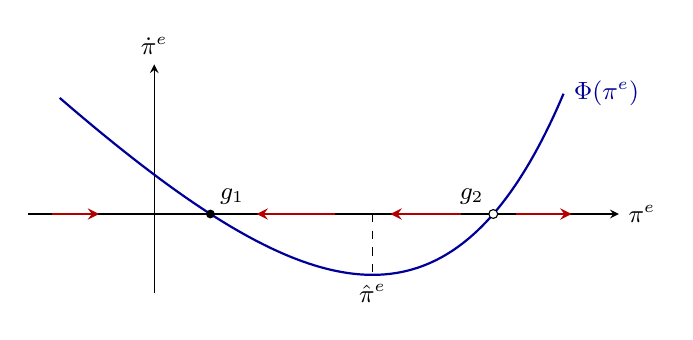
\begin{tikzpicture}[x=2cm,y=2cm,>=stealth,font=\small]
\draw[->] (-0.8,0) -- (2.95,0) node[right] {$\pi^e$};
\draw[->] (0,-0.5) -- (0,0.95) node[above] {$\dot\pi^e$};
\draw[thick,blue!60!black,domain=-0.6:2.6,samples=80,smooth] plot (\x,{0.25*exp(\x)-\x})
  node[right] {$\Phi(\pi^e)$};
\draw[dashed] (1.386,0) -- (1.386,-0.386) node[below] {$\hat\pi^e$};
\fill (0.357,0) circle (1.6pt) node[above right] {$g_1$};
\draw[fill=white] (2.153,0) circle (1.6pt) node[above left] {$g_2$};
\draw[->,thick,red!70!black] (-0.65,0) -- (-0.35,0);
\draw[->,thick,red!70!black] (1.15,0) -- (0.65,0);
\draw[->,thick,red!70!black] (1.95,0) -- (1.5,0);
\draw[->,thick,red!70!black] (2.3,0) -- (2.65,0);
\end{tikzpicture}
\end{center}

\passo{Dynamics of $m$}{$m=Ce^{-b\pi^e}$ moves opposite to $\pi^e$. From $\pi^e(0)<g_2$, $m$
converges monotonically to $m_1=G/g_1$, where $g_M=\pi=\pi^e=g_1$. From $\pi^e(0)>g_2$, $S(\pi^e)$
keeps falling as $\pi^e$ rises, so $\dot m\le-\tfrac{b\beta}{1-b\beta}[G-S(\pi^e(0))]<0$ and $m$
collapses in finite time, as in (b).}

\intuicao{Between $g_1$ and $g_2$, steady-state revenue at the expected rate exceeds $G$, so the
government needs $g_M=G/m<\pi^e$; by (4) actual inflation falls short of expectations, which are
revised down toward $g_1$. Above $g_2$ the base erodes faster than the rate rises: the required $g_M$
exceeds $\pi^e$, inflation outruns expectations, and the economy slides into hyperinflation. The
high-inflation steady state is a threshold, not an outcome, which is why the text focuses on $g_1$.}

\armadilha{If $\beta>1/b$, the factor $\beta/(1-b\beta)$ in (3) is negative and every arrow reverses:
in (b) $\pi^e$ falls forever (explosive deflation), and in (c) $g_2$ is stable and $g_1$ unstable,
the ``peculiar'' case of Romer's footnote 34.}

\refbib{Romer (2012), \S11.9, eqs.~(11.67)--(11.75), Figs.~11.8--11.10 and footnotes 33--34;
Cagan (1956).}

\checado{\texttt{check-11-22-6-16.py} re-derives (3) and (4) with sympy from the two equations,
confirms that (3) reproduces (11.75) and that $\min\Phi=\frac{\beta}{b(1-b\beta)}\ln(G/S^{\mathrm{MAX}})$;
for $C=b=1$, $\beta=\tfrac12$ it checks $G=\tfrac12$: $\Phi>0$ on a grid and the simulated $\pi^e$ passes
30 ($m<10^{-13}$) at $t\approx4.75$, before $\bar t\approx7.57$; and $G=\tfrac14$: $S(g_i)=G$, $\Phi'(g_1)<0<\Phi'(g_2)$, paths from below $g_1$
and from $(g_1,g_2)$ converge to $g_1$ and the path from above $g_2$ explodes. The solution manual
agrees with (3), with (b) and with the stability ranking in (c), but its text for (c) has a sign typo:
for $\pi^e$ outside $[g_1,g_2]$ it writes $\dot\pi^e<0$; it must be $\dot\pi^e>0$, as its own eq.~(11)
and the arrows in its figure require.}
